\documentclass[utf8x, 12pt]{G7-32}

% Настройки стиля ГОСТ 7-32
% Для начала определяем, хотим мы или нет, чтобы рисунки и таблицы нумеровались в пределах раздела, или нам нужна сквозная нумерация.
\EqInChapter % формулы будут нумероваться в пределах раздела
\TableInChapter % таблицы будут нумероваться в пределах раздела
\PicInChapter % рисунки будут нумероваться в пределах раздела
\usepackage{slashbox}

\usepackage[table,xcdraw]{xcolor}

% Добавляем гипертекстовое оглавление в PDF
\usepackage[
bookmarks=true, colorlinks=true, unicode=true,
urlcolor=black,linkcolor=black, anchorcolor=black,
citecolor=black, menucolor=black, filecolor=black,
]{hyperref}

% Изменение начертания шрифта --- после чего выглядит таймсоподобно.
% \usepackage{cyrtimespatched}

% графика
\usepackage{graphicx}
\graphicspath{ {./img/} }

% отделять первую строку раздела абзацным отступом
\usepackage{indentfirst} 

% Пакет Tikz
\usepackage{tikz}
\usetikzlibrary{arrows,positioning,shadows}

% Произвольная нумерация списков.
\usepackage{enumerate}

% ячейки в несколько строчек
\usepackage{multirow}

% itemize внутри tabular
\usepackage{paralist,array}

% объявляем новую команду для переноса строки внутри ячейки таблицы
\newcommand{\specialcell}[2][c]{%
	\begin{tabular}[#1]{@{}c@{}}#2\end{tabular}}

\usepackage{tikz}
\usepackage{pgfplots}
\usepackage{pdfpages}
\usepackage{caption}
\usepackage{longtable}
% \captionsetup[table]{position=top}
% Листинги

\usepackage{listings}
\usepackage{caption}

\usepackage{courier}
\usepackage{wrapfig}

\usepackage{xcolor}
\captionsetup[lstlisting]{singlelinecheck=off, justification=raggedright}


\definecolor{codegreen}{rgb}{0,0.6,0}
\definecolor{codegray}{rgb}{0.5,0.5,0.5}
\definecolor{codepurple}{rgb}{0.58,0,0.82}
\definecolor{backcolour}{rgb}{0.95,0.95,0.92}


% Значения по умолчанию
\lstset{
  % подсветка синтаксиса
  backgroundcolor=\color{backcolour},   
  commentstyle=\color{codegreen},
  keywordstyle=\color{magenta},
  numberstyle=\tiny\color{codegray},
  stringstyle=\color{codepurple},
  basicstyle= \footnotesize,
  breakatwhitespace=true,% разрыв строк только на whitespacce
  breaklines=true,       % переносить длинные строки
%   captionpos=b,          % подписи снизу -- вроде не надо
  inputencoding=koi8-r,
  numbers=left,          % нумерация слева
  numberstyle=\footnotesize,
  showspaces=false,      % показывать пробелы подчеркиваниями -- идиотизм 70-х годов
  showstringspaces=false,
  showtabs=false,        % и табы тоже
  stepnumber=1,
  tabsize=4,              % кому нужны табы по 8 символов?
  frame=single,
  escapeinside={(*}{*)}, %выделение
  literate={а}{{\selectfont\char224}}1
  {б}{{\selectfont\char225}}1
  {в}{{\selectfont\char226}}1
  {г}{{\selectfont\char227}}1
  {д}{{\selectfont\char228}}1
  {е}{{\selectfont\char229}}1
  {ё}{{\"e}}1
  {ж}{{\selectfont\char230}}1
  {з}{{\selectfont\char231}}1
  {и}{{\selectfont\char232}}1
  {й}{{\selectfont\char233}}1
  {к}{{\selectfont\char234}}1
  {л}{{\selectfont\char235}}1
  {м}{{\selectfont\char236}}1
  {н}{{\selectfont\char237}}1
  {о}{{\selectfont\char238}}1
  {п}{{\selectfont\char239}}1
  {р}{{\selectfont\char240}}1
  {с}{{\selectfont\char241}}1
  {т}{{\selectfont\char242}}1
  {у}{{\selectfont\char243}}1
  {ф}{{\selectfont\char244}}1
  {х}{{\selectfont\char245}}1
  {ц}{{\selectfont\char246}}1
  {ч}{{\selectfont\char247}}1
  {ш}{{\selectfont\char248}}1
  {щ}{{\selectfont\char249}}1
  {ъ}{{\selectfont\char250}}1
  {ы}{{\selectfont\char251}}1
  {ь}{{\selectfont\char252}}1
  {э}{{\selectfont\char253}}1
  {ю}{{\selectfont\char254}}1
  {я}{{\selectfont\char255}}1
  {А}{{\selectfont\char192}}1
  {Б}{{\selectfont\char193}}1
  {В}{{\selectfont\char194}}1
  {Г}{{\selectfont\char195}}1
  {Д}{{\selectfont\char196}}1
  {Е}{{\selectfont\char197}}1
  {Ё}{{\"E}}1
  {Ж}{{\selectfont\char198}}1
  {З}{{\selectfont\char199}}1
  {И}{{\selectfont\char200}}1
  {Й}{{\selectfont\char201}}1
  {К}{{\selectfont\char202}}1
  {Л}{{\selectfont\char203}}1
  {М}{{\selectfont\char204}}1
  {Н}{{\selectfont\char205}}1
  {О}{{\selectfont\char206}}1
  {П}{{\selectfont\char207}}1
  {Р}{{\selectfont\char208}}1
  {С}{{\selectfont\char209}}1
  {Т}{{\selectfont\char210}}1
  {У}{{\selectfont\char211}}1
  {Ф}{{\selectfont\char212}}1
  {Х}{{\selectfont\char213}}1
  {Ц}{{\selectfont\char214}}1
  {Ч}{{\selectfont\char215}}1
  {Ш}{{\selectfont\char216}}1
  {Щ}{{\selectfont\char217}}1
  {Ъ}{{\selectfont\char218}}1
  {Ы}{{\selectfont\char219}}1
  {Ь}{{\selectfont\char220}}1
  {Э}{{\selectfont\char221}}1
  {Ю}{{\selectfont\char222}}1
  {Я}{{\selectfont\char223}}1
}

\lstloadlanguages{
  C++
}

% Стиль для псевдокода: строчки обычно короткие, поэтому размер шрифта побольше
\lstdefinestyle{pseudocode}{
  basicstyle=\small,
  keywordstyle=\color{black}\bfseries\underbar,
  language=Pseudocode,
  numberstyle=\footnotesize,
  commentstyle=\footnotesize\it
}

% Стиль для обычного кода: маленький шрифт
\lstdefinestyle{realcode}{
  basicstyle=\scriptsize,
  numberstyle=\footnotesize
}

% Стиль для коротких кусков обычного кода: средний шрифт
\lstdefinestyle{simplecode}{
  basicstyle=\footnotesize,
  numberstyle=\footnotesize
}

% Стиль для BNF
\lstdefinestyle{grammar}{
  basicstyle=\footnotesize,
  numberstyle=\footnotesize,
  stringstyle=\bfseries\ttfamily,
  language=BNF
}

% Определим свой язык для написания псевдокодов на основе Python
\lstdefinelanguage[]{Pseudocode}[]{Python}{
  morekeywords={each,empty,wait,do},% ключевые слова добавлять сюда
  morecomment=[s]{\{}{\}},% комменты {а-ля Pascal} смотрятся нагляднее
  literate=% а сюда добавлять операторы, которые хотите отображать как мат. символы
    {->}{\ensuremath{$\rightarrow$}~}2%
    {<-}{\ensuremath{$\leftarrow$}~}2%
    {:=}{\ensuremath{$\leftarrow$}~}2%
    {<--}{\ensuremath{$\Longleftarrow$}~}2%
}[keywords,comments]

% Свой язык для задания грамматик в BNF
\lstdefinelanguage[]{BNF}[]{}{
  morekeywords={},
  morecomment=[s]{@}{@},
  morestring=[b]",%
  literate=%
    {->}{\ensuremath{$\rightarrow$}~}2%
    {*}{\ensuremath{$^*$}~}2%
    {+}{\ensuremath{$^+$}~}2%
    {|}{\ensuremath{$|$}~}2%
}[keywords,comments,strings]

% Подписи к листингам на русском языке.
\renewcommand\lstlistingname{\cyr\CYRL\cyri\cyrs\cyrt\cyri\cyrn\cyrg}
\renewcommand\lstlistlistingname{\cyr\CYRL\cyri\cyrs\cyrt\cyri\cyrn\cyrg\cyri}



\begin{document}

\frontmatter % выключает нумерацию ВСЕГО; здесь начинаются ненумерованные главы: реферат, введение, глоссарий, сокращения и прочее.

\begin{table}[ht]
	\centering
	\begin{tabular}{|c|p{400pt}|} 
	\hline
		\begin{tabular}[c]{@{}c@{}} 
\includegraphics[scale=0.37]{EmblemBMSTU} \\\end{tabular} &
		\footnotesize\begin{tabular}[c]{@{}c@{}}\textbf{Министерство~науки~и~высшего~образования~Российской~Федерации}\\\textbf{Федеральное~государственное~бюджетное~образовательное~учреждение}\\\textbf{~высшего~образования}\\\textbf{«Московский~государственный~технический~университет}\\\textbf{имени~Н.Э.~Баумана}\\\textbf{(национальный~исследовательский~университет)»}\\\textbf{(МГТУ~им.~Н.Э.~Баумана)}\\\end{tabular}  \\
	\hline
	\end{tabular}
\end{table}
\noindent\rule{\textwidth}{4pt}
\noindent\rule[14pt]{\textwidth}{1pt}
\hfill 
\noindent
\makebox{ФАКУЛЬТЕТ~}%
\makebox[\textwidth][l]{\underline{~~~~«Информатика и системы управления»~~~~~~~~~~~~~~~~~~~~~~~~~~~~~~~~~~~~~~~~~~~~}}%
\\
\noindent
\makebox{КАФЕДРА~}%
\makebox[\textwidth][l]{\underline{~~~~~~~«Программное обеспечение ЭВМ и информационные технологии»~~~~~~~~}}%
\\


\begin{center}
	\vspace{3cm}
	{\bf\huge Отчёт\par}
	{\bf\Large по лабораторной работе №1\par}
	\vspace{0.5cm}
\end{center}


\noindent
\makebox{\large{\bf Название:}~~~}
\makebox[\textwidth][l]{\large\underline{~Расстояния Левенштейна и Дамерау-Левенштейна~~~~~~~~~~~~~}}\\

\noindent
\makebox{\large{\bf Дисциплина:}~~~}
\makebox[\textwidth][l]{\large\underline{~Анализ алгоритмов~~~~~~~~~~~~~~~~~~~~~~~~~~~~~~~~~~~~~~~~~~~~~~~~~~~~}}\\

\vspace{1.5cm}
\noindent
\begin{tabular}{l c c c c c}
    Студент      & ~ИУ7-55Б~               & \hspace{3.5cm} & \hspace{3.5cm}                 & &  М.А. Козлов \\\cline{2-2}\cline{4-4} \cline{6-6} 
    \hspace{3cm} & {\footnotesize(Группа)} &                & {\footnotesize(Подпись, дата)} & & {\footnotesize(И.О. Фамилия)}
\end{tabular}

\vspace{1cm}

\noindent
\begin{tabular}{l c c c c}
    Преподователь & \hspace{6cm}   & \hspace{3.5cm}                 & & Л.Л. Волкова \\\cline{3-3} \cline{5-5} 
    \hspace{3cm}  &                & {\footnotesize(Подпись, дата)} & & {\footnotesize(И.О. Фамилия)}
\end{tabular}

\begin{center}	
	\vfill
	\large \textit {Москва, 2020}
\end{center}

\thispagestyle {empty}
\pagebreak

\tableofcontents
\pagebreak

\Introduction
    В данной работе требуется изучить и применить алгоритмы нахождения 
    расстояния Левенштейна и Дамерау-Левенштейна, а также получить
    практические навыки реализации указанных алгоритмов.
    
    Расстояния Левенштейна и Дамерау-Левенштейна применяется для следующих задач: \begin{enumerate}
        \item для автозамены, в том числе в поисковых системах;
        \item в биоинформатике для сравнения цепочек белков, генов и т.д.
    \end{enumerate}
\newpage

\mainmatter % это включает нумерацию глав и секций в документе ниже

\chapter{ Аналитический раздел}
\label{cha:analytical}
    В данной части будут рассмотрены теоретические 
    основы задачи коммивояжера и муравьиного алгоритма. 
	
    \section{Постановка задачи коммивояжера} 
        Коммивояжёр (фр. commis voyageur) -- бродячий торговец.
        Коммивояжёру, чтобы распродать нужные и не очень нужные в хозяйстве товары,
        необходимо объехать n пунктов и в конце концов вернуться в исходный пункт.
        Требуется определить наиболее выгодный маршрут объезда. 
        В качестве меры выгодности маршрута (точнее говоря, невыгодности)
        может служить суммарное время в пути, суммарная стоимость дороги,
        или, в простейшем случае, длина маршрута.
        
        Задача коммивояжёра -- важная задача транспортной логистики,
        отрасли, занимающейся планированием транспортных перевозок.
        В терминах теории графа она формулируется как задача
        поиска минимального по стоимости замкнутого маршрута
        по всем вершинам без повторений на полном взвешенном 
        графе с n вершинами. 
        Где вершины графа являются городами, которые должен
        посетить коммивояжер, а веса ребер отражают расстояния
        или стоимости проезда \cite{rec-alg}. 
        
    \section{Метод полного перебора}
        Задача коммивояжёра может быть решена перебором всех вариантов объезда и выбором оптимального.
        Но точный переборный алгоритм её решения имеет факториальную сложность, так как
        количество возможных маршрутов очень быстро возрастает с ростом n. 
        Оно равно n! — количеству способов упорядочения пунктов. 
        К примеру, для 100 пунктов количество вариантов будет представляться 158-значным числом.
        Мощная ЭВМ, способная перебирать миллион вариантов в секунду, 
        будет биться с задачей на протяжении примерно 3*10144 лет.
        Не спасает ситуацию даже то, что для каждого варианта маршрута имеется 2n равноценных,
        отличающихся выбором начального пункта (n вариантов) и направлением обхода (2 варианта).
        Перебор с учётом этого сокращается незначительно. 
        Для проверки оптимальности маршрута необходимо проверить 
        его со всеми имеющимися, что невозможно за полиномиальное время,
        поэтому задача коммивояжёра является NP-трудной.

    \section{Муравьиный алгоритм}
        Все муравьиные алгоритмы базируются на моделировании поведения колонии муравьев.
        Колония муравьев может рассматриваться как многоагентная система,
        в которой каждый агент (муравей) функционирует автономнопо очень простым правилам.
        В противовес почти примитивному поведению агентов, 
        поведение всей системы получается на удивление разумным.
            
        Муравьиные алгоритмы представляют собой вероятностную жадную эвристику,
        где вероятности устанавливаются, 
        исходя из информации о качестве решения,
        полученной из предыдущих решений.
        
        Идея муравьиного алгоритма -- моделирование поведения муравьёв,
        связанного с их способностью быстро находить кратчайший путь от муравейника
        к источнику пищи и адаптироваться к изменяющимся условиям,
        находя новый кратчайший путь. 
        При своём движении муравей метит путь феромоном,
        и эта информация используется другими муравьями для выбора пути.
        Это элементарное правило поведения и определяет способность муравьёв 
        находить новый путь, если старый оказывается недоступным.
        
        Какие же механизмы обеспечивают столь сложное поведение муравьев,
        и что можем мы позаимствовать у этих крошечных существ для решения 
        своих глобальных задач? Основу «социального» поведения муравьев 
        составляет самоорганизация -- множество динамических механизмов,
        обеспечивающих достижение системой глобальной цели 
        в результате низкоуровневого взаимодействия ее элементов.
        Принципиальной особенностью такого взаимодействия является 
        использование элементами системы только локальной информации.
        При этом исключается любое централизованное управление и
        обращениек глобальному образу, репрезентирующему систему во внешнем мире.
        Самоорганизация является результатом взаимодействия 
        следующих четырех компонентов:
        \begin{enumerate}
            \item случайность;
            \item многократность;
            \item положительная обратная связь;
            \item отрицательная обратная связь.
        \end{enumerate}
        
        Рассмотрим случай, когда на оптимальном доселе пути возникает преграда.
        В этом случае необходимо определение нового оптимального пути. 
        Дойдя до преграды, муравьи с равной вероятностью будут обходить её справа и слева. 
        То же самое будет происходить и на обратной стороне преграды. 
        Однако, те муравьи, которые случайно выберут кратчайший путь,
        будут быстрее его проходить, и за несколько передвижений он 
        будет более обогащён феромоном.
        Поскольку движение муравьёв определяется концентрацией феромона,
        то следующие будут предпочитать именно этот путь, 
        продолжая обогащать его феромоном до тех пор,
        пока этот путь по какой-либо причине не станет недоступен.
        
        Очевидная положительная обратная связь быстро приведёт к тому,
        что кратчайший путь станет единственным маршрутом движения большинства муравьёв.
        Моделирование испарения феромона -- отрицательной обратной связи -- гарантирует,
        что найденное локально оптимальное решение не будет единственным -- муравьи
        будут искать и другие пути. 
        Если мы моделируем процесс такого поведения на некотором графе, 
        рёбра которого представляют собой возможные пути перемещения муравьёв,
        в течение определённого времени, то наиболее обогащённый феромоном путь 
        по рёбрам этого графа и будет являться решением задачи, 
        полученным с помощью муравьиного алгоритма.
        
        Обобщим все выше сказанное. 
        Любой муравьиный алгоритм, независимо от модификаций, представим в следующем виде:
        \begin{enumerate}
            \item создание муравьев;
            \item поиск решения;
            \item обновление феромона;
            \item дополнительные действия (опиционально).
        \end{enumerate}
        
        Рассмотрим каждый шаг в цикле более подробно.
        
        \subsection{Создание муравьев}
            Стартовая точка, куда помещается муравей, 
            зависит ограничений, накладываемых условиями задачи. 
            Потому что для каждой задачи способ размещения муравьёв
            является определяющим. Либо все они помещаются в одну точку,
            либо в разные с повторения, либо без повторений.

            На этом же этапе задается начальный уровень феромона. 
            Он инициализируется небольшим положительным числом для того, 
            чтобы на начальном шаге вероятности перехода в следующую вершину не были нулевыми.
            
        \subsection{Поиск решения}
            Вероятность перехода из вершины i в вершину j определяется по формуле (\ref{equation:probability:way}):
            
            \begin{equation}
                p_{i,j}={\frac{(\tau_{i,j}^{\alpha })(\eta_{i,j}^{\beta})}{\sum(\tau_{i,j}^{\alpha})(\eta_{i,j}^{\beta})}},
                \label{equation:probability:way} 
            \end{equation}
                
            где $\tau_{i,j}$ -- расстояние от города i до j;
                
            $\eta_{i,j}$ -- количество феромонов на ребре ij;
            
            $\alpha$ -- параметр влияния длины пути;
            
            $\beta$ -- параметр влияния феромона.
        
        
        \subsection{Обновление феромона}
            После того, как муравей успешно проходит маршрут, 
            он оставляет на всех пройденных ребрах след, 
            обратно пропорциональный длине пройденного пути. 
            Новый след феромона вычисляется по формуле (\ref{equation:track}):
            \begin{equation}
                \tau _{i,j}=(1-\rho)\tau_{i,j}+\Delta\tau_{i,j},
                \label{equation:track} 
            \end{equation}
            
            где $ \rho_{i,j}$ --доля феромона, который испарится;
            
            $\tau_{i,j}$ -- количество феромона на дуге ij;
                
            $\Delta\tau_{i,j}$ -- количество отложенного феромона.
            
        \subsection{Дополнительные действия} 
            Обычно здесь используется алгоритм локального поиска,
            однако он может также появиться и после поиска всех решений. 
        
    \section{Муравьиный алгоритм в задаче коммивояжера}
        Рассмотрим, как реализовать четыре составляющие самоорганизации муравьев при оптимизации маршрута коммивояжера.
        Многократность взаимодействия реализуется итерационным поиском маршрута коммивояжера одновременно несколькими муравьями.
        При этом каждый муравей рассматривается как отдельный, независимый коммивояжер, решающий свою задачу. 
        За одну итерацию алгоритма каждый муравей совершаетполный маршрут коммивояжера. 
        Положительная обратная связь реализуется как имитация поведения муравьев 
        типа «оставление следов -- перемещение по следам». 
        Чем больше следов оставлено на тропе -- ребре графа в задаче коммивояжера,
        тем больше муравьев будет передвигаться по ней. 
        При этом на тропе появляются новые следы, привлекающие дополнительных муравьев.
        Для задачи коммивояжера положительная обратная связь реализуется следующим стохастическим правилом: 
        вероятность включения ребра графа в маршрут муравья пропорциональна количеству феромона на нем.
		
        С учетом особенностей задачи коммивояжёра, 
        мы можем описать локальные правила поведения муравьев при выборе пути.

        Муравьи имеют собственную «память».
        Поскольку каждый город может быть посещён только один раз,
        то у каждого муравья есть список уже посещенных городов -- список запретов. 
        Обозначим через $ J $ список городов, 
        которые необходимо посетить муравью $k$,
        находящемуся в городе $i$.
        
        Муравьи обладают «зрением» -- видимость есть эвристическое желание посетить город $j$,
        если муравей находится в городе $i$. 
        Будем считать, что видимость обратно пропорциональна расстоянию между городами.

        Муравьи обладают «обонянием» -- они могут улавливать след феромона,
        подтверждающий желание посетить город $j$ из города $i$ на основании опыта других муравьёв.
        Количество феромона на ребре $(i,j)$ в момент времени $t$ обозначим через $tau_{i,j}(t)$.
        На этом основании мы можем сформулировать вероятностнопропорциональное правило,
        определяющее вероятность перехода $k$-ого муравья из города $i$  в город $j$. 

        Пройдя ребро $(i,j)$, муравей откладывает на нём некоторое количество феромона,
        которое должно быть связано с оптимальностью сделанного выбора.
        Пусть $T_{k}(t)$ есть маршрут, пройденный муравьем $k$ к моменту 
        времени $t$ , $L_{k} (t)$ - длина этого маршрута, 
        а $Q$ -- параметр, имеющий значение порядка длины оптимального пути. 
        Тогда откладываемое количество феромона может быть задано формулой (\ref{equation:delta:pheromone:Q}):

        \begin{equation}
            {\displaystyle \Delta\tau_{i,j}^k={
            \begin{cases}
                Q/L_{k}& {\text{если k-ый муравей прошел по ребру ij;}}\\
                0&{\text{иначе,}}
            \end{cases}}}
            \label{equation:delta:pheromone:Q} 
        \end{equation}
        
        где Q -- количество феромона, переносимого муравьем.
        
        С учётом этого приходим к окончательному варианту формулы (\ref{equation:delta:pheromone}):
        \begin{equation}
            \Delta \tau_{i,j}= \tau_{i,j}^0 + \tau_{i,j}^1 + ... + \tau_{i,j}^k,
            \label{equation:delta:pheromone}
        \end{equation}
       
        где k -- количество муравьев в вершине графа с индексами i и j.
    
        
\newpage
\chapter{ Констукторский раздел}
\label{cha:design}
    разработка алгоритма и его схема, 
    требования к функциональности ПО,
    наметить тесты 

    ПО должно вводить 2 строчки, выводить расстояние и кроме
    2 матрицу, осуществлять замеры проц. времени t [и памяти]
\newpage
\chapter{ Технологический раздел}
\label{cha:technological}

    В данном разделе будут выбраны средства реплизации ПО и представлен листинг кода. 

    \section{Средства реализации}
        В данной работе используется язык программирования C++, так как
        язык позволяет написать программу, работающую относительно быстро. 
        Проект выполнен в IDE Visual Studio 2019 \cite{visual-studio}.

        Для замера процессорного времени была использована функция QueryPerformanceCounter \cite{QueryPerformanceCounter} 
        из библиотеки WinAPI, использование которой представлено в листинге \ref{lst:QueryPerformanceCounter}.

        \begin{lstlisting}[language=C++, label=lst:QueryPerformanceCounter, caption=Функция замера времени]
using funcDL = std::size_t( * )(const char*, const char* );
double getTime(funcDL getDL, const char* s1, const char* s2, int samples)
{
    LARGE_INTEGER StartingTime, EndingTime, ElapsedMicroseconds;
    LARGE_INTEGER Frequency;

    QueryPerformanceFrequency(&Frequency);
    QueryPerformanceCounter(&StartingTime);

    // Activity to be timed
    for (size_t i = 0; i < samples; i++)
        getDL(s1, s2);

    QueryPerformanceCounter(&EndingTime);
    ElapsedMicroseconds.QuadPart = EndingTime.QuadPart - StartingTime.QuadPart;

    ElapsedMicroseconds.QuadPart *= 1000000;
    ElapsedMicroseconds.QuadPart /= (Frequency.QuadPart * samples);
    return ElapsedMicroseconds.QuadPart;
}
        \end{lstlisting}

    \section{Листинг программы}
        Ниже представлены листинги кода поиска растояния Левенштейна: \begin{enumerate}
            \item нерекурсивного с заполнением матрицы (листинг \ref{lst:matr:Levenstein});
            \item рекурсивного без заполнения матрицы (листинг \ref{lst:rec:Levenstein});
            \item рекурсивного с заполнением матрицы (листинг \ref{lst:rec-matr:Levenstein});
        \end{enumerate}
        
        и код функции поиска растояния Дамерау-Левенштейна (листинг \ref{lst:matr:Dameray-Levenstein}).

        \begin{lstlisting}[language=C++, label=lst:matr:Levenstein, caption=Функция нерекурсивного поиска с заполнением матрицы]
std::size_t getLevMatr(const char* s1, const char* s2)
{
        auto n = strlen(s1);
        auto m = strlen(s2);
        auto matr = Matrix(n + 1, m + 1);

        for (size_t i = 0; i <= n; i++)
                matr[i][0] = i;

        for (size_t j = 1; j <= m; j++)
                matr[0][j] = j;

        for (size_t i = 1; i <= n; i++)
        {
                for (size_t j = 1; j <= m; j++)
                {
                        matr[i][j] = _min(_min(
                                matr[i - 1][j] + 1,
                                matr[i][j - 1] + 1),
                                matr[i - 1][j - 1] + (s1[i - 1] != s2[j - 1])
                        );
                }
        }

        return matr[n][m];
}
        \end{lstlisting}

        \begin{lstlisting}[language=C++, label=lst:rec:Levenstein, caption=Функция рекурсивного поиска без заполнения матрицы]
std::size_t getLevRec(const char* s1, const char* s2)
{
        std::size_t i = strlen(s1);
        std::size_t j = strlen(s2);
        return _getLevRec(s1, i, s2, j);
}
std::size_t _getLevRec(const char* s1, size_t i, const char* s2, size_t j)
{
	std::size_t d;
	if (i == 0)
		d = j;
	else if (j == 0)
		d = i;
	else
	{
		d = _min(_min(
			_getLevRec(s1, i, s2, j - 1) + 1,
			_getLevRec(s1, i - 1, s2, j) + 1),
			_getLevRec(s1, i - 1, s2, j - 1) + (s1[i - 1] != s2[j - 1])
		);
	}
	return d;
}
        \end{lstlisting}

        \begin{lstlisting}[language=C++, label=lst:rec-matr:Levenstein, caption=Функция рекурсивного поиска с заполнением матрицы]
std::size_t getLevRecMatr(const char* s1, const char* s2)
{
    std::size_t n = strlen(s1);
    std::size_t m = strlen(s2);
    auto matr = Matrix(n + 1, m + 1);
    for (size_t i = 0; i < n + 1; i++)
        for (size_t j = 0; j < m + 1; j++)
            matr[i][j] = -1;
    return _getLevRecMatr(s1, n, s2, m, matr);
}
std::size_t _getLevRecMatr(const char* s1, size_t i, const char* s2, size_t j, Matrix& matr)
{
	if (i == 0)
		matr[i][j] = j;
	else if (j == 0)
		matr[i][j] = i;
	else
	{
		if (matr[i][j - 1] == -1)
			matr[i][j - 1] = _getLevRecMatr(s1, i, s2, j - 1, matr);
		if (matr[i - 1][j] == -1)
			matr[i - 1][j] = _getLevRecMatr(s1, i - 1, s2, j, matr);
		if (matr[i - 1][j - 1] == -1)
			matr[i - 1][j - 1] = _getLevRecMatr(s1, i - 1, s2, j - 1, matr);
		matr[i][j] = _min(_min(matr[i][j - 1], matr[i - 1][j]) + 1, matr[i - 1][j - 1] + (s1[i - 1] != s2[j - 1]));
	}

	return matr[i][j];
}
        \end{lstlisting}

        \begin{lstlisting}[language=C++, label=lst:matr:Dameray-Levenstein, caption=Функция поиска растояния Дамерау-Левенштейна]
std::size_t getDamLevMatr(const char* s1, const char* s2)
{
    std::size_t n = strlen(s1);
    std::size_t m = strlen(s2);
    auto matr = Matrix(n + 1, m + 1);
    
    for (size_t i = 0; i <= n; i++)
        matr[i][0] = i;

    for (size_t j = 1; j <= m; j++)
        matr[0][j] = j;

    for (size_t i = 1; i <= n; i++)
    {
        for (size_t j = 1; j <= m; j++)
        {
            matr[i][j] = _min(_min(
                matr[i - 1][j] + 1,
                matr[i][j - 1] + 1),
                matr[i - 1][j - 1] + (s1[i - 1] != s2[j - 1]
            ));

            if (i > 1 && j > 1 && s1[i - 1] == s2[j - 2] && s1[i - 2] == s2[j - 1])
                matr[i][j] = _min(matr[i][j], matr[i - 2][j - 2] + 1);
        }
    }

    return matr[n][m];
}
        \end{lstlisting}
    
        
    \section{Тестирование}
        В таблице \ref{table:testing} отображён возможный набор тестов
        для тестирования методом чёрного ящика, результаты которого, 
        представленные на рисунке \ref{png:testing:result}, подтверждают
        прохождение программы перечисленных тестов.
        \begin{table}[]
            \caption{Тесты проверки корректности программы}
            \centering
            \begin{tabular}{|c|c|c|c|c|}
            \hline
            № & строка 1 & строка 2 & \begin{tabular}[c]{@{}c@{}}Ожидаемый результат \\ (р.Л, р.Д-Л)\end{tabular} & \begin{tabular}[c]{@{}c@{}}Фактический результат\\ (р.Л, р.Д-Л)\end{tabular} \\ \hline
            1 & 0        & 0        & 0, 0                                                                        & 0, 0                                                                         \\ \hline
            2 & 0        & ab       & 2, 2                                                                        & 2, 2                                                                         \\ \hline
            3 & abba     & baab     & 3, 2                                                                        & 3, 2                                                                         \\ \hline
            4 & abcd     & qwer     & 4, 4                                                                        & 4, 4                                                                         \\ \hline
            \end{tabular}
            \label{table:testing}
        \end{table}

        \begin{figure}[h!]
            \centering
            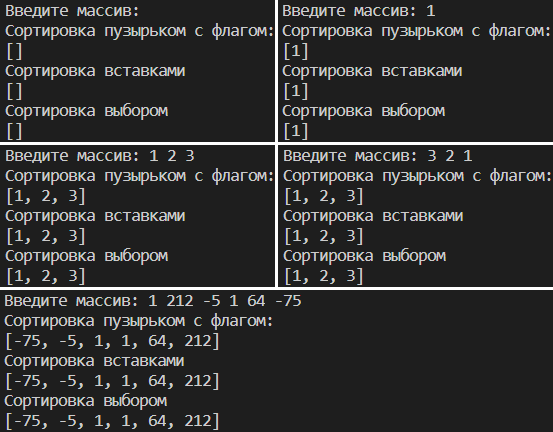
\includegraphics[scale=1.2]{testing.png}
            \caption{Результаты тестирования}
            \label{png:testing:result}
        \end{figure}

    \section{Сравнительный анализ потребляемой памяти}
        Для проведения анализов будем считать, что размер int - 4 байта,
        % size_t - 4 байта.

\newpage
\chapter{Экспериментальный раздел}
\label{cha:research}
    В данном разделе будут проведены эксперименты для проведения 
    сравнительного анализа алгоритмов по затрачиваемому процессорному 
    времени\cite{CPU-time} и количеству максимально затрачиваемой памяти.

    \section{Сравнительный анализ на основе замеров времени работы алгоритмов}
    
        Был проведён замер времени работы каждого из алгоритмов:
        
        1) на небольших длинах строк (рисунок \ref{png:test:1});
        
        2) на относительно больших длинах строк (рисунок \ref{png:test:2}).
        
        Ниже предствалены графики полученных замеров времени
        (диаграммы \ref{diag:test:1} и \ref{diag:test:2}).

        \begin{figure}[h!]
            \centering
            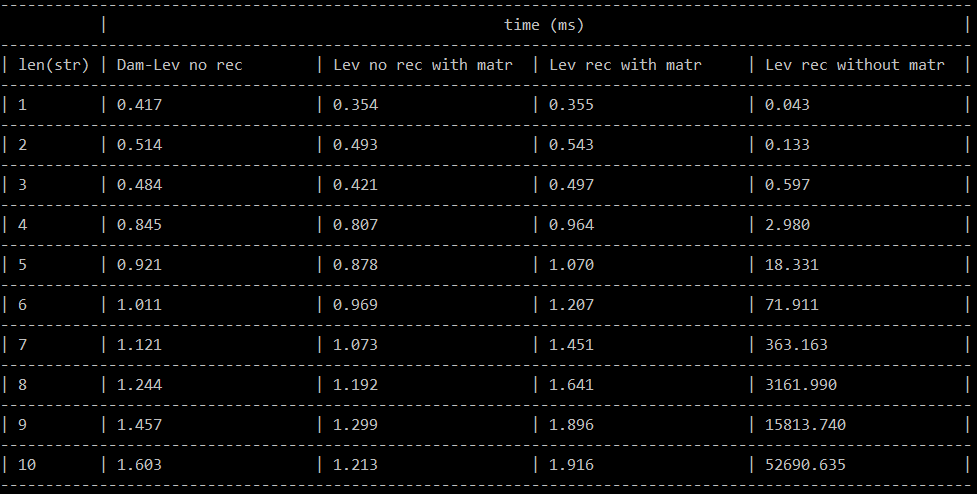
\includegraphics[scale=0.7]{test1.png}
            \caption{Результаты замера времени на маленьких строках}
            \label{png:test:1}

            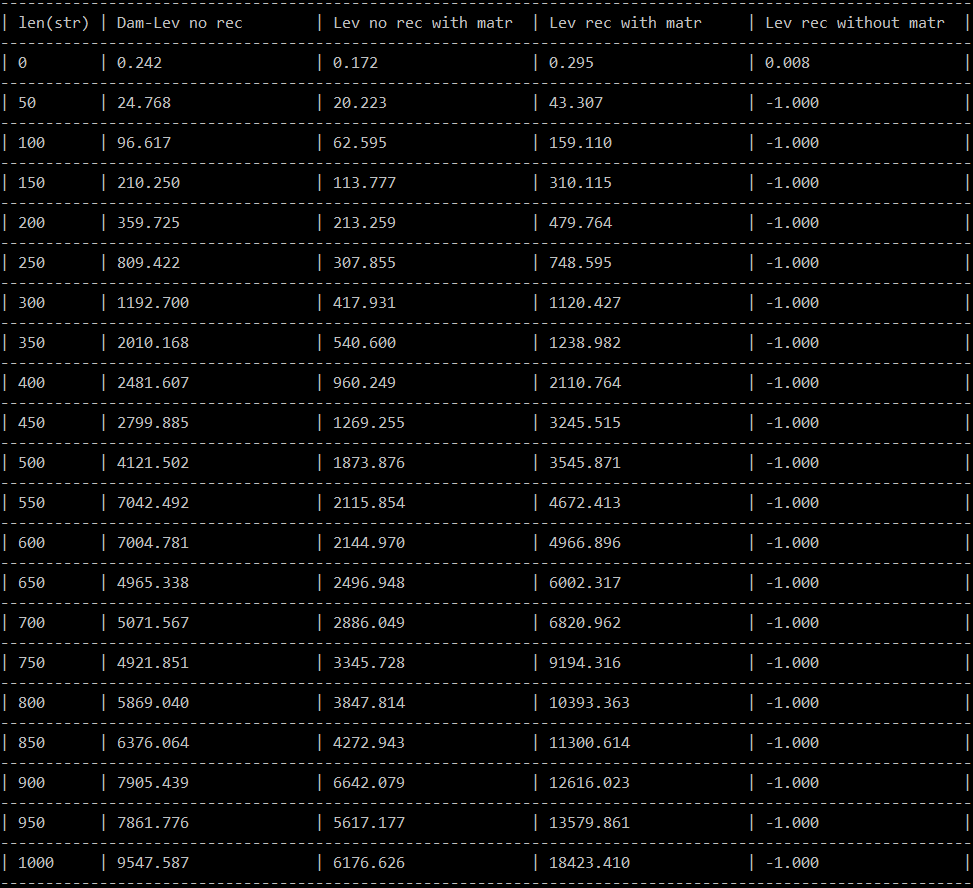
\includegraphics[scale=0.7]{test2.png}
            \caption{Результаты замера времени на больших строках}
            \label{png:test:2}
        \end{figure}

        \begin{figure}[h!]
            \centering
            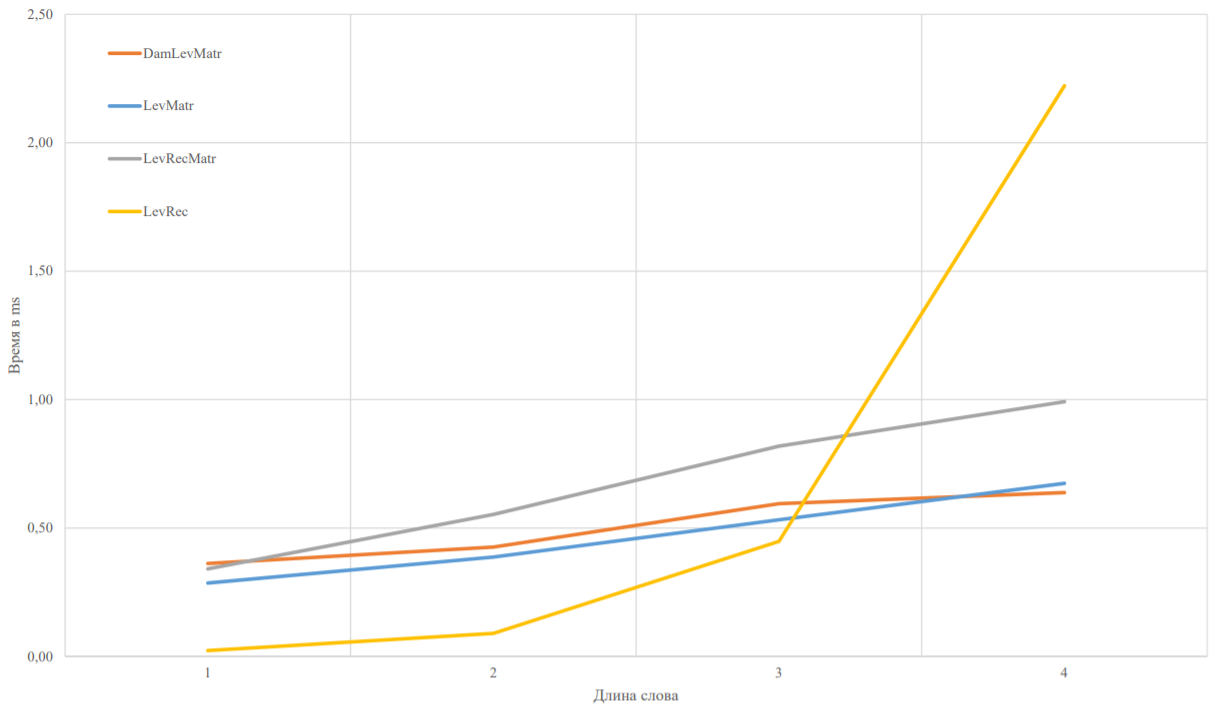
\includegraphics[scale=0.7]{diagram1.png}
            \caption{Зависимость времени работы алгоритма от длины малых строк}
            \label{diag:test:1}
            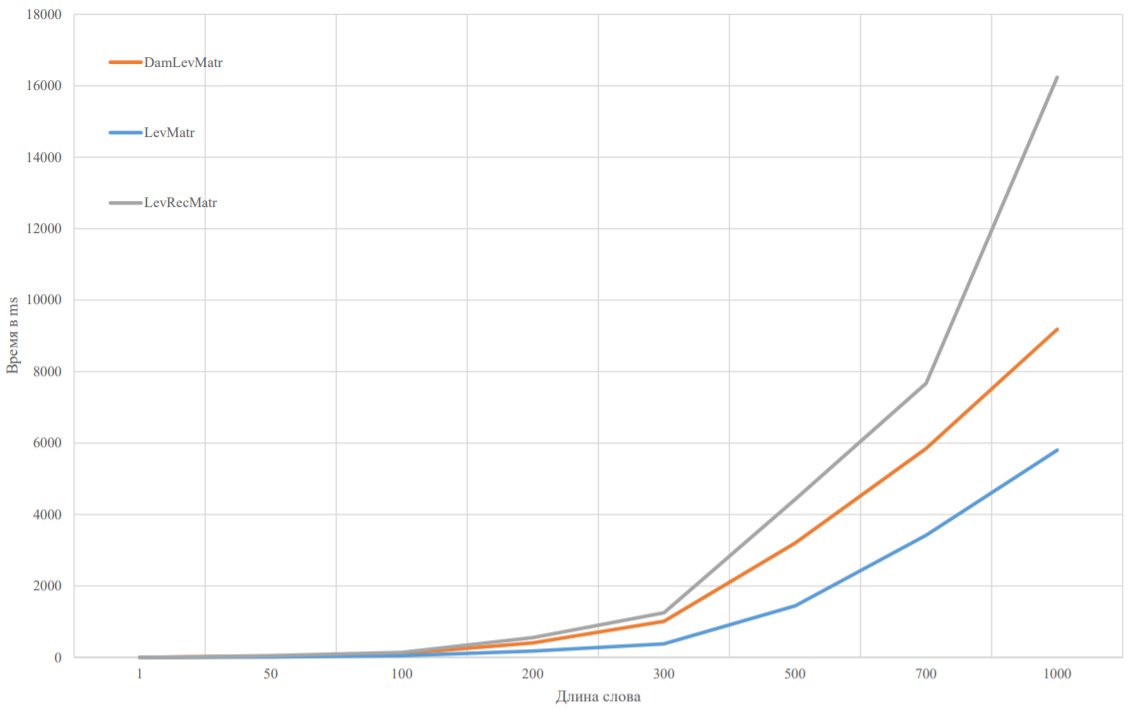
\includegraphics[scale=0.7]{diagram2.png}
            \caption{Зависимость времени работы алгоритма от длины больших строк}
            \label{diag:test:2}
        \end{figure}

        \vspace{1cm}

        Visual studio позволяет оценить затраты динамической памяти, через профилирование heap.
        Ниже выделение матрицы 10х10
        \begin{figure}[h!]
            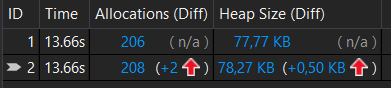
\includegraphics{use_heap_memory.png}
        \end{figure}
\newpage

\backmatter % Здесь заканчивается нумерованная часть документа и начинаются ссылки и
\Conclusion
    В ходе выполнения лабораторной работы 
    были описаны и реализованы алгоритмы конвейерной обработки.
    Разработанный конвейер, с параллельно работающими линиями,
    позволил ускорить работу программы в 2,6 раз
    по сравнению с линейной реализацией. 
    Однако если одна из стадий намного более трудоемкая, чем остальные,
    то конвейерная обработка становится неэффективной,
    так как производительность всей программы будет упираться в производительность этой стадии,
    и разница между обычной обработкой и конвейерной будет малозаметна.
    В таком случае можно либо разбить трудоемкую стадию на набор менее трудоемких,
    либо выбрать другой алгоритм, либо отказаться от конвейерной обработки.

\bibliographystyle{gost780u}
\bibliography{report}

\end{document}